\chapter[Algoritmo Proposto]{Algoritmo Proposto}

O algoritmo proposto para a solução descrita neste sistema baseia-se em uma técnica clássica de super-resolução \cite{garcia2013tecnicas}.

O termo super-resolução (SR) é usado para descrever processos que procuram acrescentar informações de alta frequência a uma imagem interpolada a partir de uma ou mais imagens disponíveis \cite{baker2002limits}\cite{park2003super}\cite{farsiu2004advances}. Este conjunto de imagens pode ser formado por imagens decimadas ou adquiridas por múltiplos sensores capturando uma mesma cena durante determinado período de tempo. Para cenas estáticas (Figuras \ref{fig:SR_1} e \ref{fig:SR_2}), as observações são relacionadas por deslocamentos globais em nível de subpixel (geralmente ocorrendo devido a posições relativas das câmeras ou movimento do próprio sensor), enquanto para cenas dinâmicas elas são relacionadas a deslocamentos de subpixel, devido ao movimento local dos próprios objetos juntamente com os deslocamentos globais conforme pode ser visualizando na Figura \ref{fig:SR_3}. Em ambos os casos, a super-resolução é utilizado para gerar a partir de um conjunto de imagens em baixa resolução ou de frames de uma sequência de vídeo uma imagem com maior resolução espacial \cite{figueira2013super}\cite{milanfar2010super}.
\\
\begin{figure}[h]
	\centering
	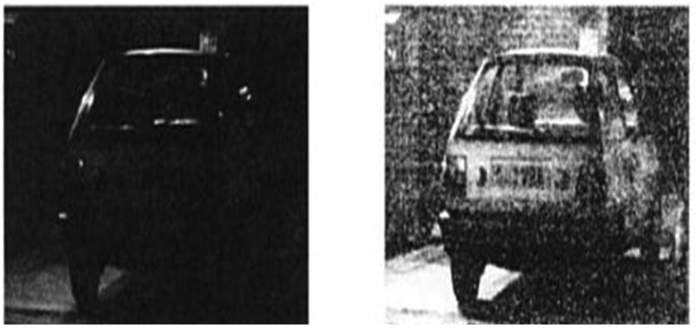
\includegraphics[scale=0.65]{figuras/SR_img_1.png}
	\caption{(esquerda) uma cena estática de uma sequência de vídeo é capturada com baixa luminosidade; (direita) após equalização de histograma a placa do automóvel continua ilegível devido ao ruído     natural da imagem \cite{kang2000digital}.}
	\label{fig:SR_1}
\end{figure}

\begin{figure}[h]
	\centering
	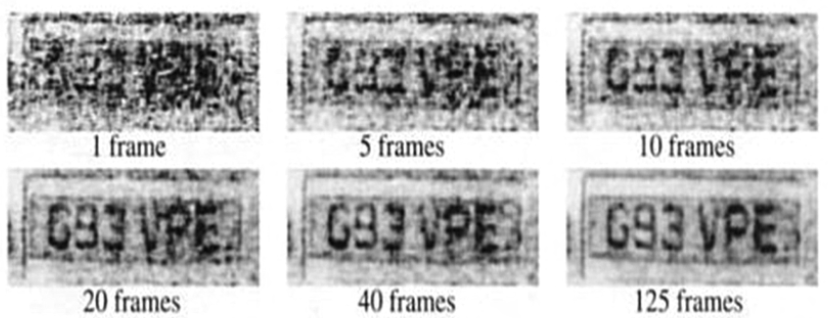
\includegraphics[scale=0.45]{figuras/SR_img_2.png}
	\caption{Legibilidade da placa como resultado da média do conjunto cada vez maior de quadros \cite{kang2000digital}.} 
	\label{fig:SR_2}
\end{figure}

\begin{figure}[h]
	\centering
	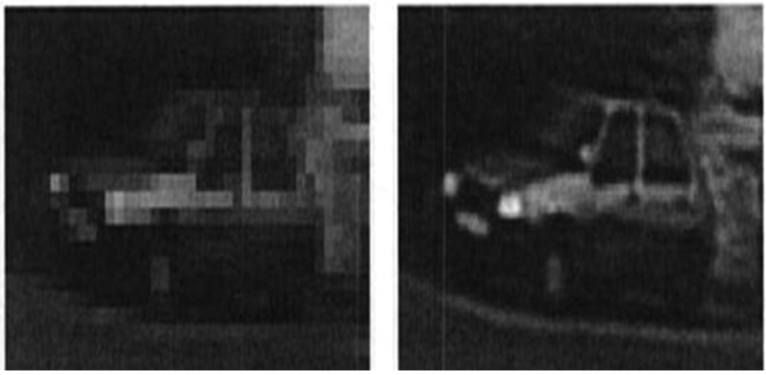
\includegraphics[scale=0.45]{figuras/img_SR_3.png}
	\caption{(esquerda) a região de interesse é capturada em uma cena dinâmica; (direita) a SR estima a cena subjacente a partir de 50 imagens. A reconstrução possui o triplo da resolução em relação à imagem original \cite{kang2000digital}.}
	\label{fig:SR_3}
\end{figure}

\subsection{Super-resolução por exemplos}

A técnica de super-resolução baseada em exemplos, busca informações de alta frequência em uma base de dados, com imagens em alta resolução, para adicionar a uma imagem interpolada. A princípio, não há relação direta entre a base de dados e a imagem de entrada, de forma que o algoritmo pode atender a uma ampla gama de imagens em baixa resolução, com um grande banco de dados \cite{freeman2002example}.

Esta técnica baseia-se no fato que a coleção de imagens que capturam cenas reais, por exemplo, possui variabilidade muito menor do que a coleção de imagens aleatórias \cite{garcia2013tecnicas}.

Na super-resolução baseada em exemplos, gera-se para cada imagem em alta resolução $I_j$ uma versão com componentes de baixa frequência, $I_j^B$, e uma versão de componentes de alta frequência, $I_j^A$, onde $I_j^A$ = $I_j$ - $I_j^B$. Assim considera-se a imagem interpolada $I_0$ correspondente somente as componentes de baixa frequência ($I_0 = I_0^B$ ), o que permite obter uma relação entre a imagem de entrada ($I_0$) e as imagens de referência ($I_j$) \cite{garcia2013tecnicas}.

De acordo com o mesmo autor, $I_0^B, I_j^B$ e $I_0^A$ são divididas em blocos regulares, e procura-se em $I^B_j$ pelo bloco mais semelhante a cada um dos blocos de $I_0^B$. De acordo com a posição do bloco escolhido em $I_j^B$, extrai-se o bloco em $I_j^A$. Este bloco de alta frequência é então somado a $I_0$, acrescentando detalhes que não pudem ser obtidos através da interpolação. Tal processo é ilustrado na Figura \ref{fig:SR_4}.

\begin{figure}[h]
	\centering
	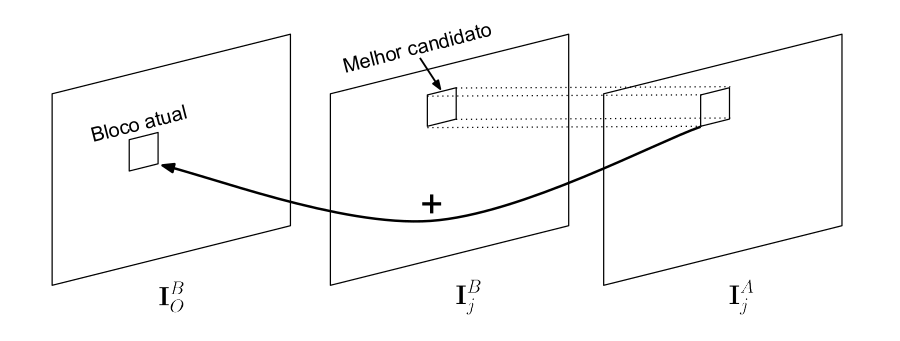
\includegraphics[scale=0.50]{figuras/superresolucao_4.png}
	\caption{Super-resolução baseada em exemplos: a imagem interpolada $I_0^B$ recebe informações de alta frequência a partir de uma imagem em alta resolução $I_j$ separada em versões com componentes de baixa e alta frequência, $I_j^B$ e $I_j^A$ \cite{garcia2013tecnicas}.}

	\label{fig:SR_4}
\end{figure}

